\section{Program Transformation}
\label{sec-opt}

After selecting the code regions to optimize, we currently manually
transform the source code to systematically enable the overlapping of
computation and communication through the following steps.


\subsection{Function outlining}

Given a loop to optimize, we first outline the computation and
communication inside the loop into separate functions, in order to
make it easier to replicate and reorder them later into different loop
iterations. In particular, we divide the statements at each iteration
I of the target loop into the MPI communications at iteration I
(Comm(I)), the computation (Before(I)) that should run before Comm(I),
and the computation (After(I)) to evaluate after Comm(I) Each group of
statements is then outlined into a separate procedure, with the loop
index variables as its function parameters.\footnote{These components
  can alternatively be simply tagged as Comm(I), Before(I), and
  After(I) if the optimization were to be fully automated; outlining
  makes it easy to modify the code manually.}  Take NAS FT in
Figure~\ref{fig:ft_loop} as an example.  The loop to optimize is
divided into $Comm(I)$, the MPI communication at iteration I;
$Before(I)$, the computation before communication at iteration I; and
$After(I)$, the computation after communication at iteration I.


\subsection{Converting MPI communications}

Each blocking MPI operation, for example, {\em alltoall} collectives
and point-to-point send-receives, is converted to an equivalent
nonblocking communication combined with a blocking wait.  For example,
in Figure~\ref{fig:ft_loop}, the outlined communication function
$Comm(I)$, which invokes $MPI\_Alltoall$ internally, is replaced by
$Icomm(I)$ and $Wait(I)$, which are the corresponding nonblocking
communication ($MPI\_Ialltoall$) and wait operations converted from
$Comm(I)$, respectively.


\subsection{Reordering computation and communication}

After the previous steps, the body of the loop to optimize now
contains a sequence of specially named operations such as $Before(I)$,
$After(I)$, $Icomm(I)$, and $Wait(I)$, where $I$ is the loop index
variable looping from $1$ to $N$.

We then \emph{interleave} the communication and computation operations
of consecutive loop iterations, as illustrated in
Figure~\ref{fig:cco:reorder}, in two steps:

\begin{enumerate}

\item Move $Before(1)$ and $Icomm(1)$ to the outside before the first
  iteration of the loop starts, and move $Wait(N)$ and $After(N)$
  outside after the last loop iteration as shown in
  Figure~\ref{fig:cco:reorder:c}.

\item Move $Before(I)$ and $Icomm(I)$ above $Wait(I-1)$ and
  $After(I-1)$ as shown in Figure~\ref{fig:cco:reorder:d}.

\end{enumerate}

After the reordering, the nonblocking communication in the current
iteration I (between $Icomm(I)$ and $Wait(I)$) can be processed in
parallel with the computation in the previous ($After(I-1)$) and next
($Before(I+1)$) iterations.


\subsection{Replicating the communication buffer}

Each MPI operation needs a dedicated buffer to hold the data being
communicated.  Applications typically first allocate the necessary
communication buffers at the initialization stage and then reuse the
same buffers in the same MPI operations across different loop
iterations.  After applying our optimization, as illustrated in
Figure~\ref{fig:cco:shift}, the communication ($Icomm(i)$ and
$Wait(i)$) at each $i$th iteration, where $i \geq 2$, is overlapped
with computation $Before(i+1)$ and $After(i-1)$.  Assuming that two
distinct buffers, {\em InBuf} and {\em OutBuf}, are used for sending
and receiving each message, respectively, each buffer needs to be
replicated into a pair of equal size to ensure that distinct buffers
are used across the overlapping iterations, as illustrated in
Figure~\ref{fig:cco:dup}.  In particular, we replicate each buffer by
allocating additional memory outside the loop and then alternately use
a distinct buffer in every pair of consecutive loop iterations.


\subsection{Inserting MPI\_Tests}

When using nonblocking MPI operations, some CPU time needs to be
allocated, by embedding $MPI\_Test$ calls in the local computation, to
ensure continuous progress of the communications.  If the local
computation is not inside a loop, we insert one or more $MPI\_Test$
calls evenly distributed into the computation.  On the other hand, if
the local computation is inside a loop, we insert $MPI\_Test$ into the
beginning of the loop body and use a conditional variable to adjust
its frequency.  The inserted code is illustrated in
Figure~\ref{fig:cco:test}.  In both cases, the frequency of
$MPI\_Test$ is empirically adjusted as the application is ported to
each architecture.

\begin{figure}
{\scriptsize
  \centering
  \begin{subfigure}[b]{.25\textwidth}
\begin{verbatim}
DO I = 1 .. N
  Before(I)
  Comm(I)
  After(I)
END DO
\end{verbatim}
    \caption{Input loop}
    \label{fig:cco:reorder:a}
    \vspace{.1in}
  \end{subfigure}
  \begin{subfigure}[b]{.25\textwidth}
\begin{verbatim}
DO I = 1 .. N
  Before(I)
  Icomm(I)
  Wait(I)
  After(I)
END DO
\end{verbatim}
    \caption{Decouple blocking comm}
    \label{fig:cco:reorder:b}
    \vspace{.1in}
  \end{subfigure}
  \begin{subfigure}[b]{.25\textwidth}
\begin{verbatim}
Before(1)
Icomm(1)
DO I = 2 .. N
  Wait(I - 1)
  After(I - 1)
  Before(I)
  Icomm(I)
END DO
Wait(N)
After(N)
\end{verbatim}
    \caption{Move first and last iterations}
    \label{fig:cco:reorder:c}
  \end{subfigure}
  \begin{subfigure}[b]{.25\textwidth}
\begin{verbatim}
Before(1)
Icomm(1)
DO I = 2 .. N
  Before(I)
  Wait(I - 1)
  Icomm(I)
  After(I - 1)
END DO
Wait(N)
After(N)
\end{verbatim}
    \caption{Interleave consequent iterations}
    \label{fig:cco:reorder:d}
  \end{subfigure}
\caption{Steps to reorder outlined communication and computation functions}
\label{fig:cco:reorder}
}
\end{figure}

\begin{figure}
{\scriptsize
  \centering
  \begin{subfigure}[b]{.20\textwidth}
\begin{verbatim}
Before(1, InBuf)
Icomm(1, InBuf)
DO I = 2 .. N
  Before(I, InBuf)
  Wait(I - 1)
  Icomm(I, InBuf
         , OutBuf)
  After(I - 1, OutBuf)
END DO
Wait(N, OutBuf)
After(N, OutBuf)
\end{verbatim}
    \caption{Original communication that uses the same input and output $Buf$}
    \label{fig:cco:dup:a}
  \end{subfigure}
  \hspace{.01in}
  \begin{subfigure}[b]{.28\textwidth}
\begin{verbatim}
Before(1, InBuf)
Icomm(1, InBuf)
DO I = 2 .. N
  Before(I, I % 2 ==  1 ? InBuf : InBuf2)
  Wait(I - 1)
  Icomm(I, I % 2 ==  0 ? InBuf : InBuf2
         , I % 2 ==  0 ? OutBuf : OutBuf2)
  After(I - 1, , I % 2 ==  1 ? InBuf : InBuf2)
END DO
Wait(N, N % 2 == 1 ? OutBuf : OutBuf2)
After(N, N % 2 == 1 ? OutBuf : OutBuf2)
\end{verbatim}
    \caption{Replicate $Buff$ with $Buff2$ of the same size}
    \label{fig:cco:dup:b}
  \end{subfigure}
\caption{Replicate communication buffers for nonblocking communication}
\label{fig:cco:dup}
}
\end{figure}

\begin{figure}[h]
{\scriptsize
\begin{verbatim}
DO I = 1 ... L
  If I % Freq == 0
    MPI_Test
  Original_computation_statements
END DO
\end{verbatim}
}
\caption{Insert MPI\_Test into the hot computation loop at specific frequency $Freq$}
\label{fig:cco:test}
\end{figure}

\begin{figure}[h]
\centering
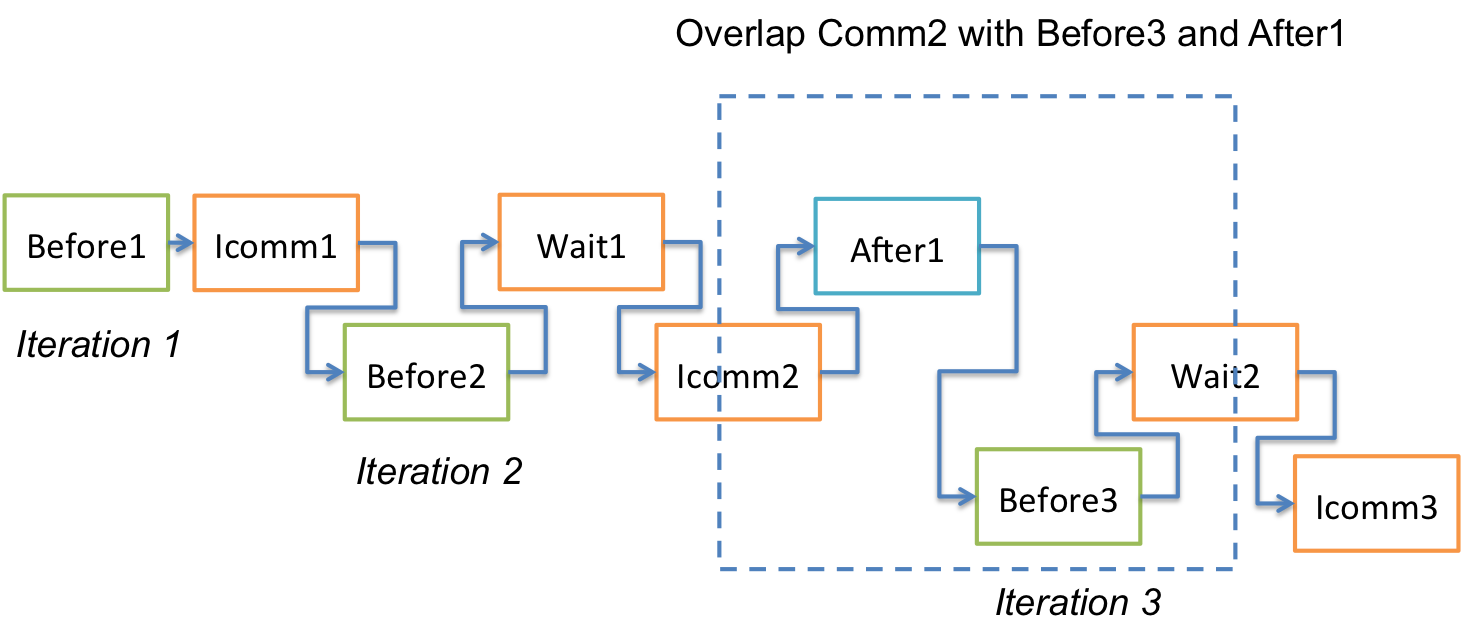
\includegraphics[width=0.49\textwidth]{fig/ft_shift.png}
\caption{Overlapped computation and communication operations}
\label{fig:cco:shift}
\end{figure}
